\section{Introduction}\label{sec:intro}

A system that rewrites its own weights, its own code or its own proofs, and keeps a rewrite when a test passes, is the basic unit of every proposal for recursive self-improvement. Good described the end point in 1965: a machine that designs a better machine, which designs a better one still, in an ``intelligence explosion'' that leaves human intelligence far behind \cite{Goo66}.\footnote{I.~J. Good, \emph{Speculations concerning the first ultraintelligent machine}, written in 1965 and printed in Advances in Computers, volume~6 (1966), pages 31--88 \cite{Goo66}. Good's argument is that an ultraintelligent machine could design better machines, so the first such machine is ``the last invention that man need ever make, provided that the machine is docile enough to tell us how to keep it under control''. The proviso is the subject of the present paper in a precise form: the docility we ask for is that every improvement the machine keeps has been checked, and we compute what the checking costs.} The literature since then has asked mostly how fast such a process could grow, under which assumptions on the returns to intelligence it reaches a vertical asymptote, and which physical limits stop it \cite{Ord26,AOA25,BSS26}. This paper asks a different question with a sharper answer: what does it cost to make sure that what the process keeps is correct?

We call the object a \emph{BLLM}, a system beyond the language model. It has three parts (Fig.~\ref{fig:architecture}). A generator, which may be a large language model \cite{VSP17,BMR20}, proposes candidate modifications of the system. A bank of randomized checks tests each candidate; a check has perfect completeness, so a correct candidate always passes, and soundness $\eps<1$, so an incorrect candidate passes one run with probability at most $\eps$. A memory keeps a candidate only after it has passed every run allotted to it, and the generator works from the memory. The word is taken from the verifier-gated engine of \cite{Bha26a}, whose escalation from token-level to beyond-token reasoning is the informal model here; the checks are the learned verifiers of \cite{CKB21,UKK22,LKB23}, the randomized identity tests of \cite{Sch80,Zip79}, the interactive and probabilistically checkable proofs of \cite{GMR89,Bab85,AS98,ALM98}, or a proof checker such as Lean \cite{MU21} run on a randomized search. The cost of a run of the check of the $i$-th candidate is $a_{i}>0$, and the schedule gives that check $r_{i}$ independent runs.

\begin{figure*}[t]
\centering
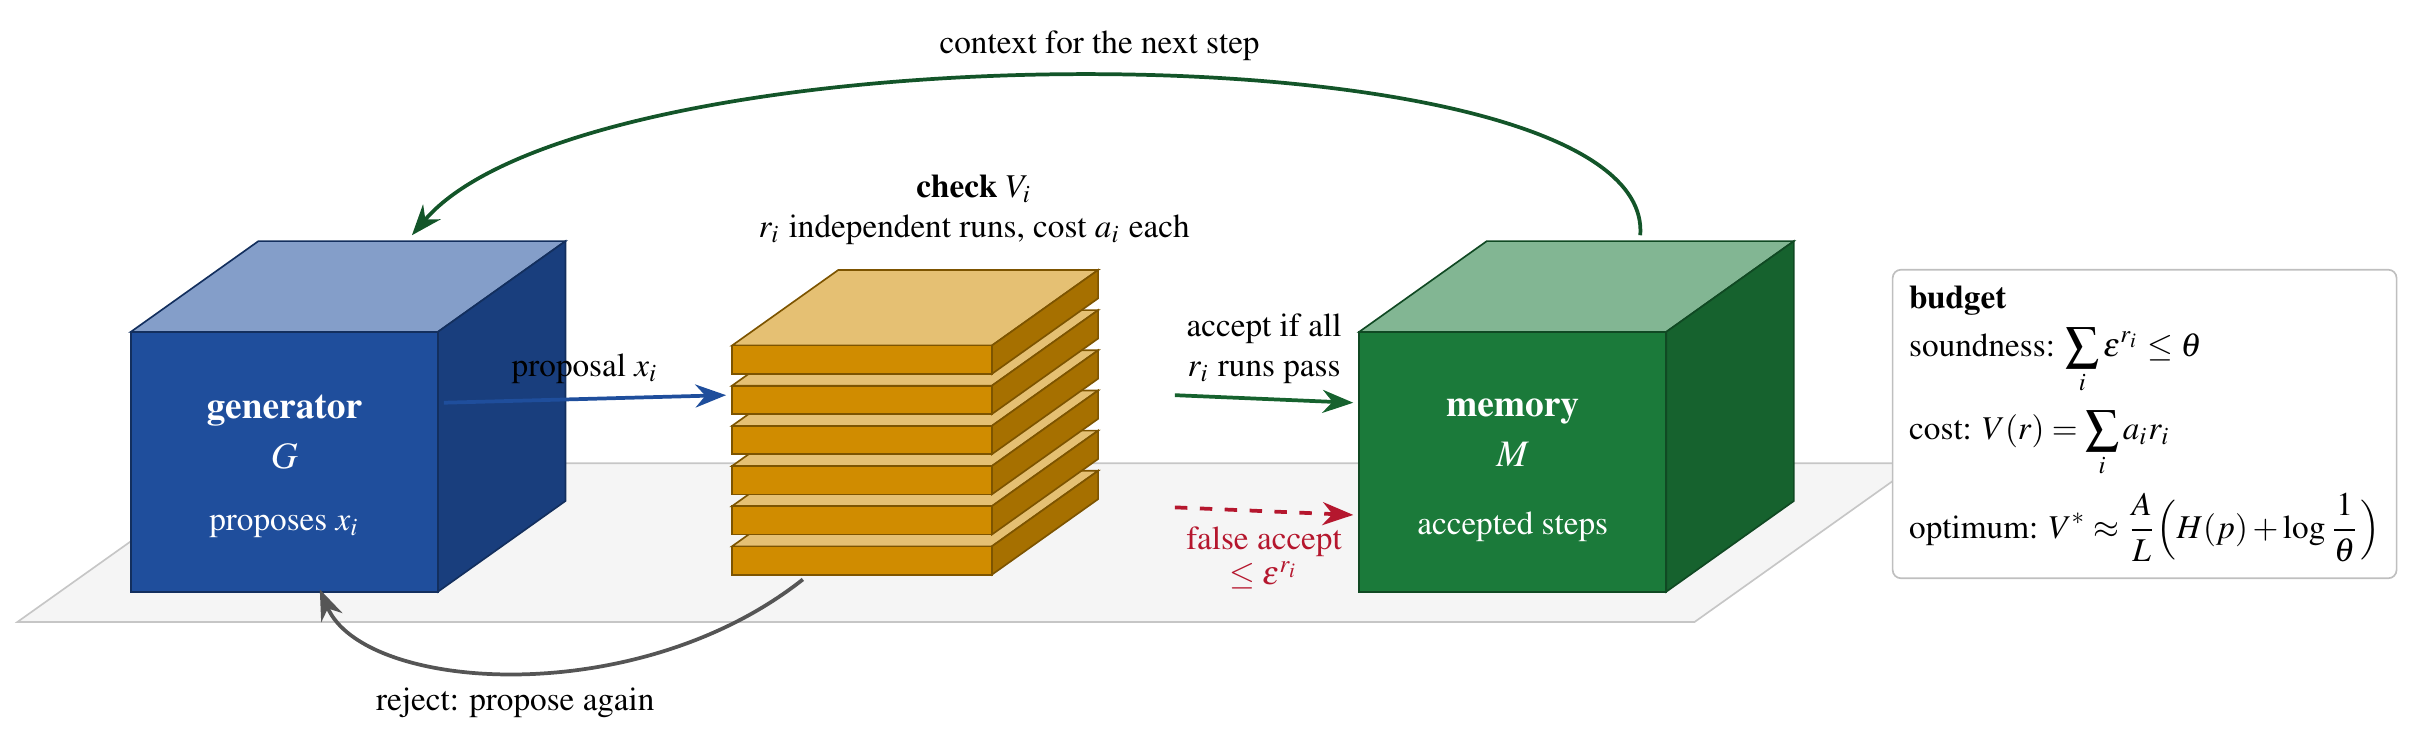
\includegraphics[width=0.94\textwidth]{figures/fig_architecture}
\caption{A BLLM. The generator proposes candidate modifications; the $i$-th candidate is tested by $r_{i}$ independent runs of a check $V_{i}$ of cost $a_{i}$ per run; an incorrect candidate survives all runs with probability at most $\eps^{r_{i}}$ and a correct one always survives; the memory keeps what survives and feeds it back as context. The budget box states the two quantities the paper controls, the expected number of false acceptances $\sum_{i}\eps^{r_{i}}\le\theta$ and the cost $V(r)=\sum_{i}a_{i}r_{i}$, and the value of the optimum (Theorem~\ref{thm:A}).}
\label{fig:architecture}
\end{figure*}

\subsection{The entropy law}

Write $A=\sum_{i}a_{i}$ for the total cost of one run of every check, $p_{i}=a_{i}/A$ for the cost profile, $H(p)=\sum_{i}p_{i}\log(1/p_{i})$ for its entropy, and $L=\log(1/\eps)$. The schedule $r$ is \emph{$\theta$-sound} when the expected number of incorrect candidates kept is at most $\theta$ in every assignment of correct and incorrect candidates, which for checks whose soundness $\eps$ is attained is the inequality $\sum_{i}\eps^{r_{i}}\le\theta$ (Section~\ref{sec:model}). Its cost is $V(r)=\sum_{i}a_{i}r_{i}$, the cost of certifying a run in which every candidate is correct, and $\Vs(\theta)$ is the least cost of a $\theta$-sound schedule.

\begin{mainthm}[Entropy law]\label{thm:A}
For $0<\theta\le1$,
\begin{equation}\label{eq:entropylaw}
\frac{A}{L}\Bigl(H(p)+\log\frac1\theta\Bigr)\ \le\ \Vs(\theta)\ \le\ \frac{A}{L}\Bigl(H(p)+\log\frac1\theta\Bigr)+A .
\end{equation}
The lower bound is attained when every $\theta p_{i}$ is an integer power of $\eps$, and the additive constant $A$ cannot be replaced by $cA$ with $c<1$. The same bounds hold for infinitely many candidates with $A<\infty$, and for schedules drawn at random independently of the checks.
\end{mainthm}

The law says that the price of soundness is an entropy. Certifying $n$ candidates of equal cost costs $(n/L)\log(n/\theta)$ up to $n$, so the tax per candidate grows like $\log n$ and not like a constant: a system that keeps more modifications must test each one harder. A skewed profile is cheaper than a flat one with the same total, because the expensive checks may be run fewer times and the cheap ones more, and the saving is measured exactly by $\log n-H(p)$. The schedule that attains the bound runs the $i$-th check $\lceil\log(A/(\theta a_{i}))/L\rceil$ times, so it spends $\log(1/p_{i})$ nats of soundness on a candidate of relative cost $p_{i}$: this is Shannon's code length \cite{Sha48}, and the analogy is exact.

\begin{mainthm}[Huffman schedules]\label{thm:C}
If $\eps=1/D$ for an integer $D\ge2$ and $\theta=D^{-k}$ for an integer $k\ge0$, then the $\theta$-sound schedules are exactly $r_{i}=\ell_{i}+k$ with $(\ell_{i})$ the lengths of a $D$-ary prefix code, and $\Vs(\theta)=A\bigl(k+L_{D}(p)\bigr)$, where $L_{D}(p)$ is the expected length of a Huffman code for $p$.
\end{mainthm}

So the optimal schedule is computed by Huffman's algorithm \cite{Huf52}, and Kraft's inequality \cite{Kra49,McM56} is the soundness condition in disguise. The additive constant of Theorem~\ref{thm:A} is the redundancy of the Huffman code, which lies in $[0,1)$ in units of $\log D$ \cite{CT06,Gal78}.

Not every check is repeated. A statistical check that averages $m$ samples and accepts when the average is close to its target has false acceptance probability of order $1/m$ by Chebyshev's inequality, not $\eps^{m}$. For a check whose cost to reach false acceptance probability $\delta$ is $a\delta^{-s}$ the entropy is replaced by a R\'enyi entropy \cite{Ren61}.

\begin{mainthm}[R\'enyi law]\label{thm:D}
For checks of polynomial order $s>0$ and $0<\theta\le1$, the least cost of a $\theta$-sound allocation is
\begin{equation}\label{eq:renyilaw}
\Vs_{s}(\theta)=\theta^{-s}\Bigl(\sum_{i}a_{i}^{1/(1+s)}\Bigr)^{1+s}=A\,\theta^{-s}e^{sH_{\alpha}(p)},
\end{equation}
where $\alpha=1/(1+s)$ and $H_{\alpha}$ is the R\'enyi entropy of order $\alpha$; and $\Vs_{s}(\theta)=A\bigl(1+s(H(p)+\log\frac1\theta)\bigr)+O(s^{2})$ as $s\to0$.
\end{mainthm}

The first-order term at $s=0$ is the entropy law, so the R\'enyi law is a one-parameter deformation of it, as Campbell's coding theorem is a deformation of Shannon's \cite{Cam65}. Section~\ref{sec:renyi} also gives a criterion, valid for every cost function, for an infinite sequence of candidates to admit a sound schedule of finite cost.

\subsection{Chains, gates and singularities}

Section~\ref{sec:chains} puts the checks into a self-improvement chain in which the generator retries a step until a candidate is kept. When each step is wrong with probability between $\rho_{\ast}>0$ and $\bar\rho<1$, the least expected cost of the chain with at most $\theta$ expected false acceptances is pinched between the entropy law at budget $\theta/\rho_{\ast}$ and the entropy law at budget $\theta(1-\bar\rho)/\bar\rho$, divided by $1-\bar\rho$ (Theorem~\ref{thm:B}). The same section proves an exponential separation between checking every step and checking only the outcome: with perfect checks the ratio of expected costs is $(1-\rho)^{-(n-1)}\ge e^{(n-1)\rho}$, and with imperfect checks the step check may accept an incorrect step with probability of order $1/n$ while the outcome check must do so with probability exponentially small in $n$ (Theorem~\ref{thm:gating}).

An infinite chain whose total expected cost is finite completes infinitely many improvements in finite cost, and we call it \emph{singular}, after the vertical asymptote of the explosion literature. It is \emph{sound} when the number $F$ of incorrect modifications it keeps is finite.

\begin{mainthm}[Sound singularities]\label{thm:E}
Let the $n$-th step cost $g_{n}$ to generate and $a_{n}\le1$ per run to check, with error probabilities in $[\rho_{\ast},\bar\rho]\subset(0,1)$, independent steps and checks of exact soundness $\eps$. Then
\begin{enumerate}[label=\textup{(\roman*)},leftmargin=2.2em,itemsep=1pt]
\item $F<\infty$ almost surely, or $\PR(F=0)>0$, if and only if $\sum_{n}\eps^{r_{n}}<\infty$, and otherwise $F=\infty$ almost surely;
\item a singular chain in which every step is checked exists if and only if $\sum_{n}g_{n}<\infty$ and $\sum_{n}a_{n}<\infty$;
\item a sound singular chain exists if and only if in addition $\sum_{n}a_{n}\log(1/a_{n})<\infty$.
\end{enumerate}
\end{mainthm}

So there is a soundness gap. For $a_{n}=1/(n\log^{\beta}n)$ a singular chain exists for every $\beta>1$, and a sound one only for $\beta>2$; between the two, every schedule fast enough to reach the asymptote keeps infinitely many errors almost surely (Corollary~\ref{cor:gap}). For a power law $a_{n}=n^{-p}$ the price of soundness, the ratio of the cheapest sound cost to the cost of one run per step, is $1/((p-1)L)+O(\log\frac1{p-1})$, and with polynomial checks of order $s$ a sound singularity exists exactly when $p>1+s$ (Fig.~\ref{fig:regimes}).

When the improvements branch, each kept improvement spawning a random number of candidates, the process is a Galton--Watson tree \cite{WG75,AN72}.

\begin{mainthm}[Branching takeoff]\label{thm:F}
Let $m$ be the mean number of correct offspring kept per kept improvement, and let the check of generation $k$ accept an incorrect candidate with probability $\delta_{k}$. Then the takeoff survives with positive probability if and only if $m>1$; the expected number of kept errors is $\mu(1-\gamma)\sum_{k\ge1}m^{k-1}\delta_{k}$; and if this series diverges then, under $\EE\,\xi\log\xi<\infty$, infinitely many errors are kept almost surely on survival. With exponential checks, soundness forces $r_{k}\ge k\log m/L$ for all large $k$, and $r_{k}=\lceil k\log(2m)/L\rceil$ suffices.
\end{mainthm}

Here $\mu$ is the mean number of candidates per kept improvement, $\gamma$ the probability that a candidate is correct and $\xi$ the number of candidates. A fixed false acceptance rate, however small, is fatal to an explosive takeoff, and the number of runs per check must grow linearly in the generation, that is, logarithmically in the size of the population: the entropy tax again.

\subsection{What the paper proves}

Table~\ref{tab:results} lists the results. The proofs are complete and elementary: the entropy law rests on the inequality $\log x\le x-1$, the R\'enyi law on H\"older's inequality, the singularity theorem on the Borel--Cantelli lemmas, and the branching theorem on the Kesten--Stigum theorem \cite{KS66} and L\'evy's conditional form of the Borel--Cantelli lemma \cite{Dur19}. Every finite inequality, the Kraft--schedule correspondence, the R\'enyi optimum, the convergence criteria for sound schedules and both Borel--Cantelli statements are proved in Lean~4 with Mathlib, in thirty-nine theorems that depend only on the three standard axioms (Appendix~\ref{app:checks}); the probabilistic limit theorems and the asymptotics of the zeta function are proved in the text and are not formalised.

The paper does not prove that any existing system is sound, and it does not predict whether an intelligence explosion will happen. Its theorems are conditional on a model, stated in Section~\ref{sec:model}: independent runs, perfect completeness, and schedules fixed in advance. Remark~\ref{rem:adaptive} shows that the last assumption matters, since a schedule allowed to stop at the first detected error escapes the entropy term at the price of discarding good work. What the paper does establish is that, inside the model, the cost of soundness is computable in closed form, that it is an entropy, and that it separates the singular processes into sound and unsound ones by a single convergent series.

\begin{table*}[t]
\caption{The main results. $A=\sum a_{i}$, $p=a/A$, $L=\log(1/\eps)$; ``Lean'' names the formalised statements of Appendix~\ref{app:checks}.}
\label{tab:results}
\centering
\footnotesize
\setlength{\tabcolsep}{4pt}
\begin{tabular}{@{}l l l >{\raggedright\arraybackslash}p{0.27\textwidth}@{}}
\toprule
Result & Statement & Proof & Lean \\
\midrule
Theorem~\ref{thm:A} & $\frac AL(H+\log\frac1\theta)\le \Vs(\theta)\le \frac AL(H+\log\frac1\theta)+A$ & Gibbs, ceilings & \lean{verification\_lower}, \lean{ceilSchedule\_cost} \\
Proposition~\ref{prop:clean} & clean runs: budgets $\theta$ and $\log\frac1{1-\theta}$ & $1-\sum q\le\prod(1-q)\le e^{-\sum q}$ & \lean{clean\_ge}, \lean{clean\_budget} \\
Proposition~\ref{prop:random} & random oblivious schedules obey Theorem~\ref{thm:A} & Jensen & \lean{randomised\_budget} \\
Proposition~\ref{prop:twosided} & two-sided checks, rate $\frac12\log\frac1{4q(1-q)}$ & Chernoff & --- \\
Theorem~\ref{thm:C} & $\Vs(D^{-k})=A(k+L_{D}(p))$ & Kraft, Huffman & \lean{kraft\_of\_schedule}, \lean{schedule\_of\_kraft} \\
Theorem~\ref{thm:D} & $\Vs_{s}(\theta)=A\theta^{-s}e^{sH_{1/(1+s)}(p)}$ & H\"older & \lean{renyi\_lower}, \lean{renyi\_attain} \\
Theorem~\ref{thm:dual} & sound schedule $\iff\sum a_{n}\psi(\lambda/a_{n})<\infty$ & Legendre duality & \lean{schedule\_of\_dual\_summable} \\
Theorem~\ref{thm:B} & chain cost between two entropy laws & Wald & \lean{entropy\_lower}, \lean{ceilSchedule\_sound} \\
Theorem~\ref{thm:gating} & step versus outcome checks: $(1-\rho)^{-(n-1)}$ & products & \lean{separation}, \lean{precision\_bounds} \\
Theorem~\ref{thm:E} & sound singularity $\iff\sum g,\sum a,\sum a\log\frac1a<\infty$ & Borel--Cantelli & \lean{sound\_schedule\_iff}, \lean{false\_accepts\_infinite} \\
Corollary~\ref{cor:gap} & soundness gap $1<\beta\le2$ & condensation & --- \\
Proposition~\ref{prop:powerlaw} & price $\sim1/((p-1)L)$ for $a_{n}=n^{-p}$ & integral comparison & --- \\
Proposition~\ref{prop:osgood} & Osgood takeoff: check time $\asymp\kappa/(c(\alpha-1)^{2}L)$ & entropy of $\zeta$ & --- \\
Theorem~\ref{thm:F} & branching takeoff and $r_{k}\ge k\log m/L$ & Kesten--Stigum, L\'evy & \lean{amplified\_summable}, \lean{contamination\_diverges} \\
\bottomrule
\end{tabular}
\end{table*}

\subsection{Organisation}

Section~\ref{sec:history} traces the three lines that meet here: self-reference and the intelligence explosion, coding and testing, and branching processes, together with the recent work on verifiers for language models. Section~\ref{sec:model} defines the model. Sections~\ref{sec:entropy} to~\ref{sec:renyi} prove the entropy law, its Huffman form and its R\'enyi deformation, with the duality criterion for infinite sequences. Section~\ref{sec:chains} treats chains and the comparison of step and outcome checks, Section~\ref{sec:singularity} the singular chains, Section~\ref{sec:branching} the branching takeoff, and Section~\ref{sec:scaling} relates the cost sequences to growth laws and to the empirical scaling laws of language models. Section~\ref{sec:status} states what is proved and what remains open. Appendix~\ref{app:derivations} collects the classical facts used, with proofs, and Appendix~\ref{app:checks} the Lean statements and the numerical checks.

Logarithms are natural unless a base is shown; $\NN=\{0,1,2,\dots\}$.
